\section{Manejo de una memoria de 32 localidades de 8 bits \label{sec:s1}}

\begin{center}
	\begin{minipage}{12cm}
		\begin{tcolorbox}[title=Actividad 1]
			Crear una memoria inicializada de 32x8 con archivo MIF como se vio en clase, habilitar la opción de uso del \textit{In-System Memory Content Editor}. Automatizar el despliegue del contenido de las 32 localidades de memoria, usando un contador a una razón de localidad por segundo. Usar la tarjeta DE2-115.
		\end{tcolorbox}	
	\end{minipage}
\end{center}

La visualización RTL de la memoria de 32 localidades de 8 bits se muestra en la \autoref{fig:mem_rtl}. De manera interna, la implementación en hardware utiliza una instancia de memoria perteneciente a la herramienta de \textit{IP Catalog} (ver \autoref{fig:mem_rtl2}). Para inicializar la memoria, se generó un archivo \textit{.mif} cuyos valores se presentan en la \autoref{fig:mem_init}, siendo estos el valor de la dirección incrementado en uno. 

La simulación se visualiza en la \autoref{fig:mem_wave}. Por cada ciclo de reloj se incrementa el valor de la dirección en uno y el valor almacenado en la localidad actual se ve reflejado en la salida Q. Una observación importante es que la señal WE esta en bajo, por lo que la memoria esta en modo lectura, siendo los datos de la memoria los observados en la \autoref{fig:mem_modelsim}. 

Con respecto a la implementación en la tarjeta DE2-115, se utilizó la herramienta \textit{In-System Memory Content Editor} para cargar la memoria de datos al FPGA, como se visualiza en la \autoref{fig:mem_content1}. En la \autoref{fig:mem_content2} se muestra que en un inicio se desconocen los valores almacenados en cada localidad, por lo que se debe hacer un chequeo utilizando la herramienta (ver \autoref{fig:mem_content3}). Realizando un monitoreo continuo, como el de la \autoref{fig:mem_content4}, se pueden ver los cambios realizados en la memoria en tiempo real.

En los Anexos se localiza la descripción de la memoria de 32 localidades de 8 bits. Al emplear un elemento proveniente de la herramienta de \textit{IP Catalog}, el código se reduce a describir las entradas y salidas y llamar a la instancia dentro del módulo principal.

\begin{figure}[ht]
	\centering
	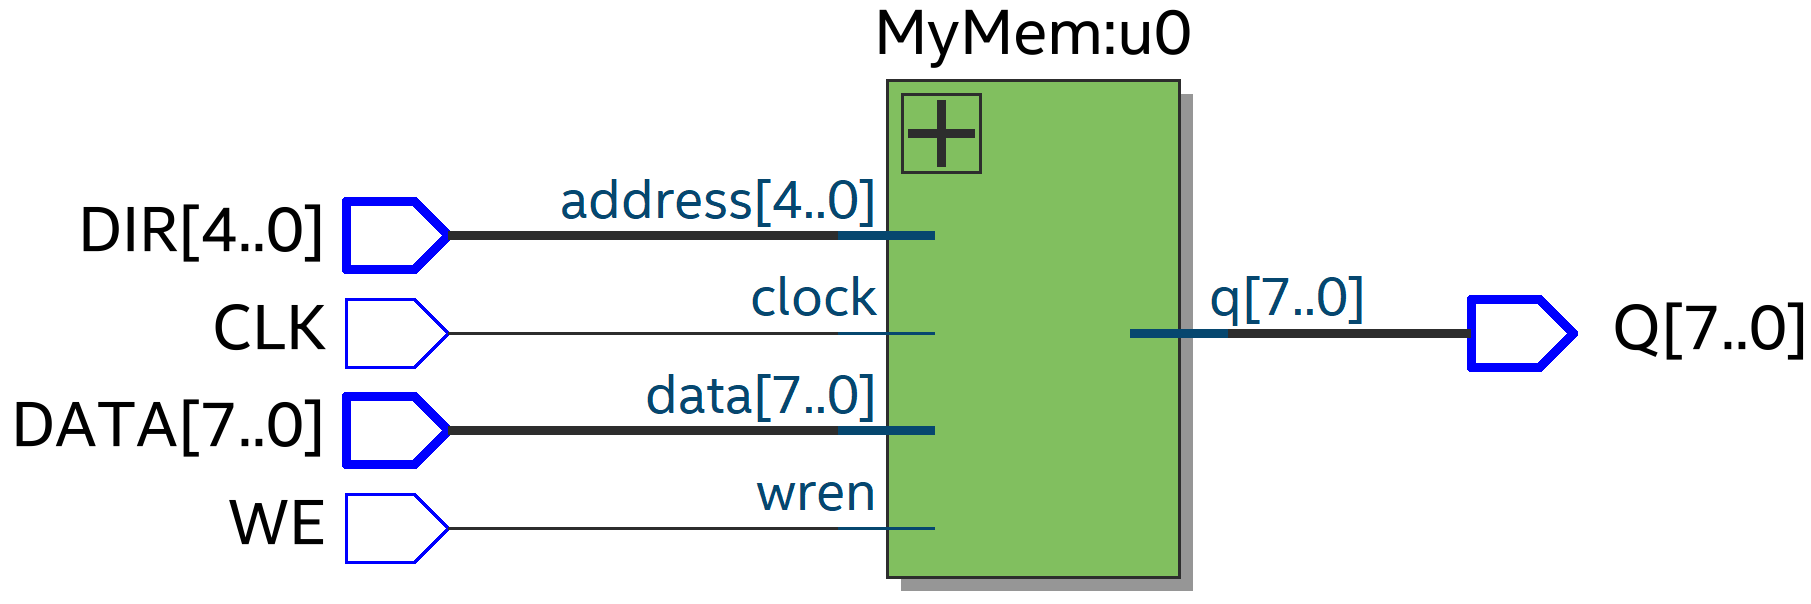
\includegraphics[scale=0.35]{Mem_RTL.png}
	\caption{Diagrama RTL de la memoria de 32 localidades de 8 bits, instanciada con un componente de IP Catalog. \label{fig:mem_rtl}}
\end{figure}

\begin{figure}[ht]
	\centering
	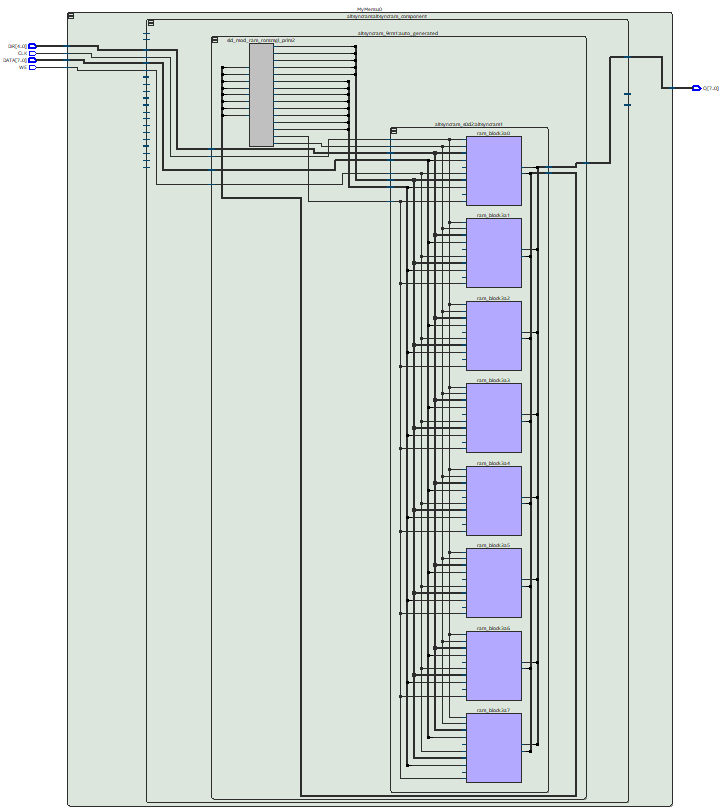
\includegraphics[scale=0.87]{Mem_RTL2.png}
	\caption{Diagrama RTL de la memoria de 32 localidades de 8 bits, instanciada con un componente de IP Catalog (vista interna). \label{fig:mem_rtl2}}
\end{figure}

\begin{figure}[ht]
	\centering
	\includegraphics[scale=1]{Mem_Init.png}
	\caption{Visualización del archivo de inicialización de la memoria de 32 localidades de 8 bits. \label{fig:mem_init}}
\end{figure}

\begin{figure}[ht]
	\centering
	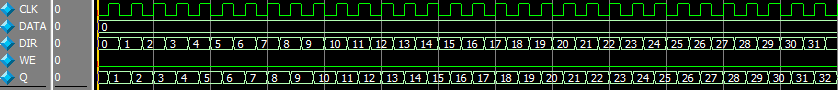
\includegraphics[scale=0.75]{Mem_Wave.png}
	\caption{Simulación de la memoria de 32 localidades de 8 bits, en el visor de formas de onda de ModelSim. \label{fig:mem_wave}}
\end{figure}

\begin{figure}[ht]
	\centering
	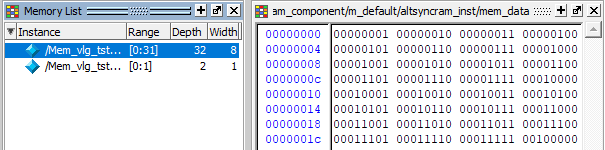
\includegraphics[scale=1]{Mem_ModelSim.png}
	\caption{Visualización de los datos de la memoria de 32 localidades de 8 bits, en la lista de memoria de ModelSim. \label{fig:mem_modelsim}}
\end{figure}

\begin{figure}[ht]
	\centering
	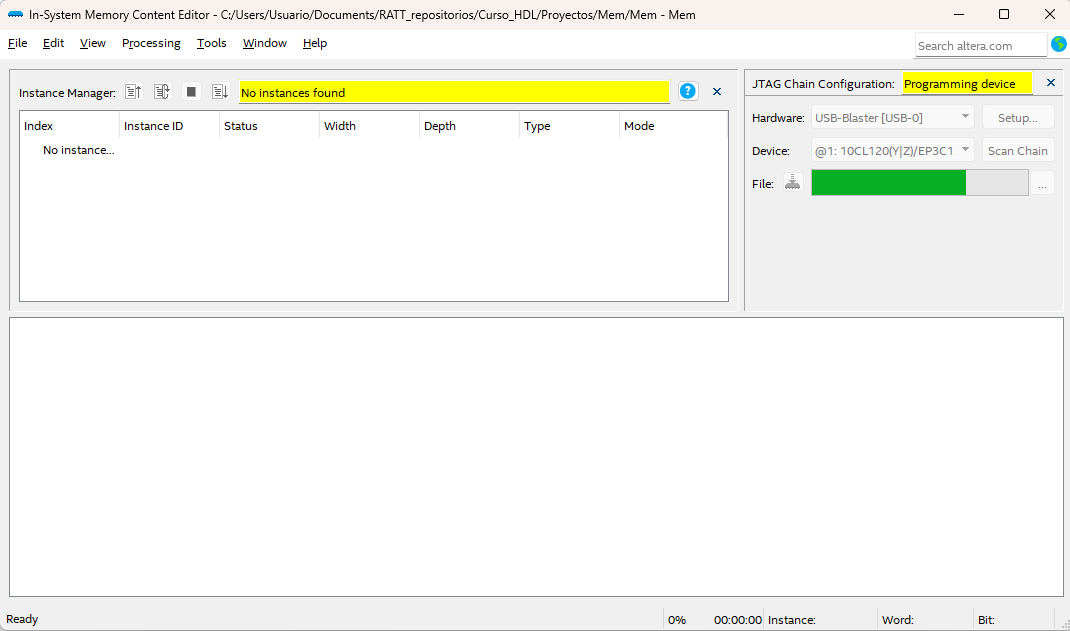
\includegraphics[scale=0.59]{Mem_Content.png}
	\caption{Uso de la herramienta \textit{In-System Memory Content Editor} para cargar la memoria al dispositivo DE2-115 (carga en progreso). \label{fig:mem_content1}}
\end{figure}

\begin{figure}[ht]
	\centering
	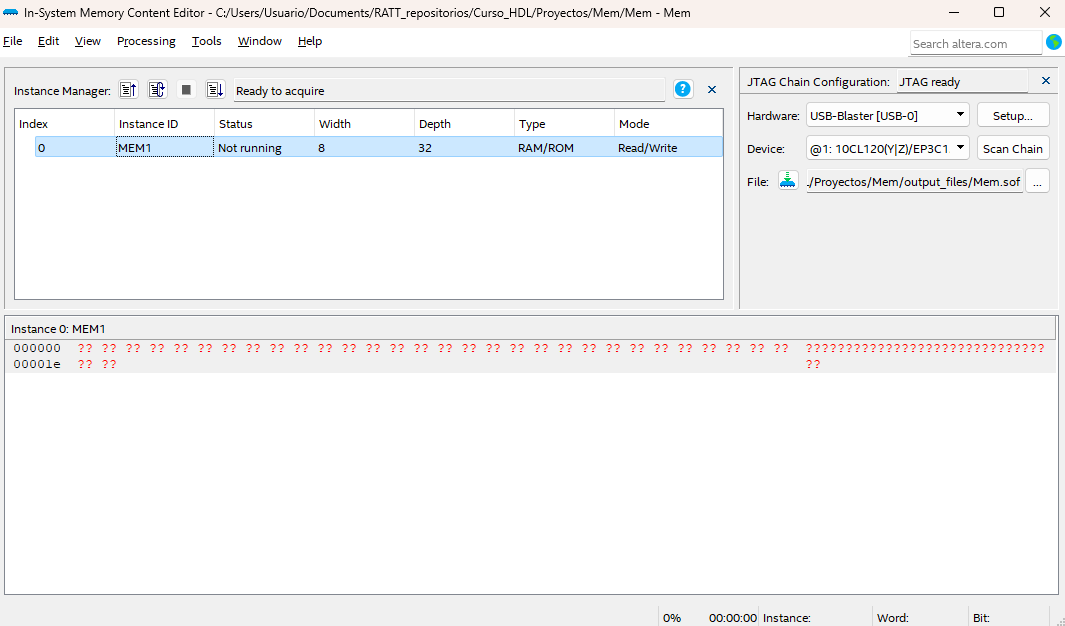
\includegraphics[scale=0.59]{Mem_Content2.png}
	\caption{Uso de la herramienta \textit{In-System Memory Content Editor} para cargar la memoria al dispositivo DE2-115 (memoria cargada). \label{fig:mem_content2}}
\end{figure}

\begin{figure}[ht]
	\centering
	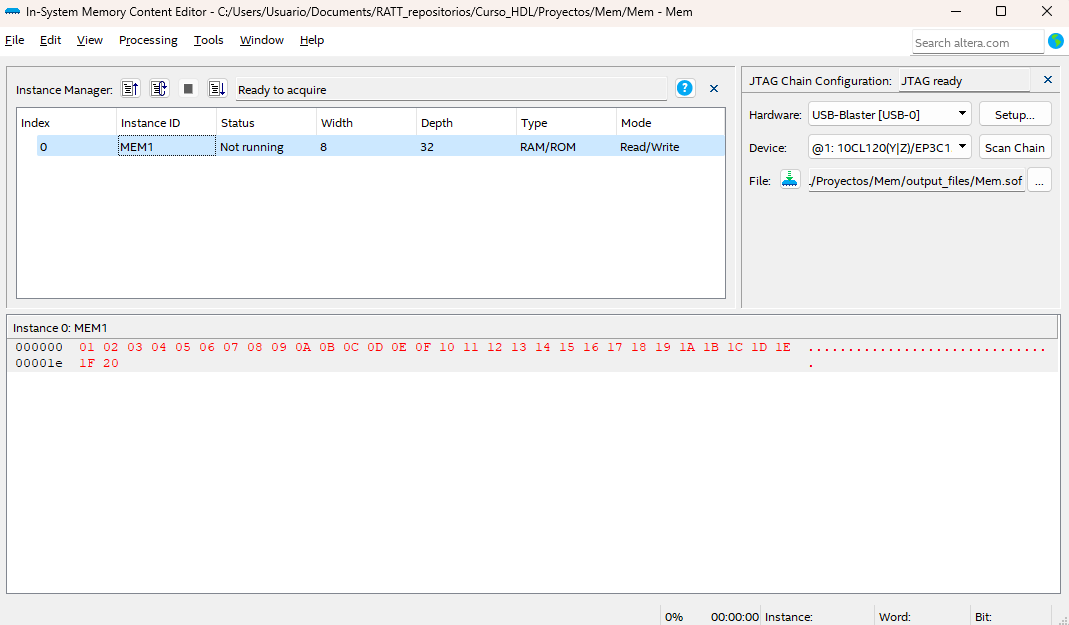
\includegraphics[scale=0.59]{Mem_Content3.png}
	\caption{Uso de la herramienta \textit{In-System Memory Content Editor} para observar los datos de la memoria en el dispositivo DE2-115 (monitoreo simple). \label{fig:mem_content3}}
\end{figure}

\begin{figure}[ht]
	\centering
	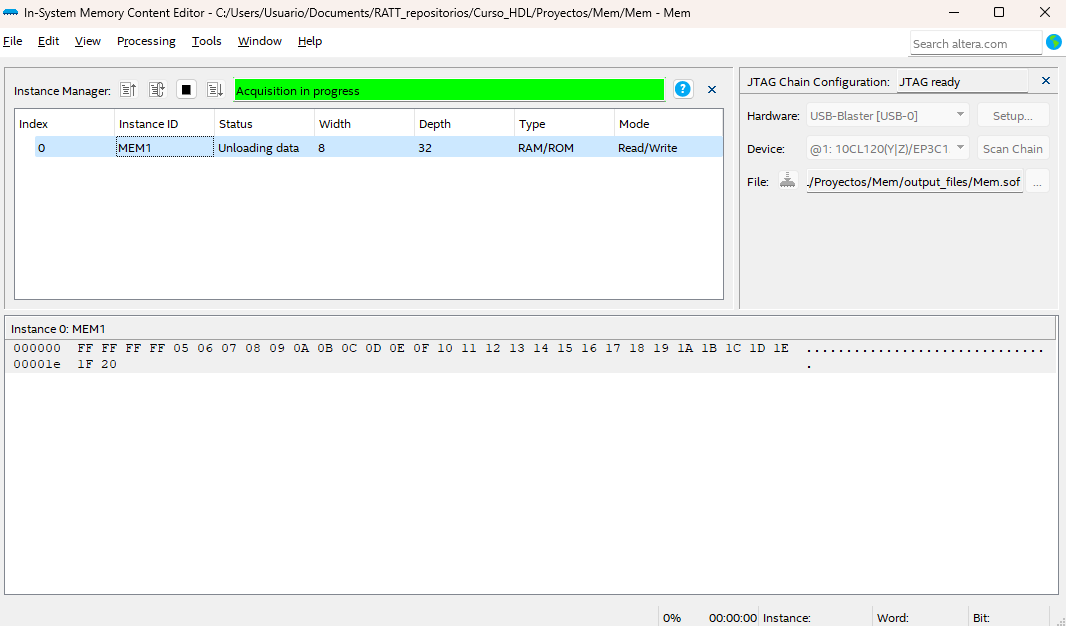
\includegraphics[scale=0.59]{Mem_Content4.png}
	\caption{Uso de la herramienta \textit{In-System Memory Content Editor} para observar los datos de la memoria en el dispositivo DE2-115 (monitoreo continuo). \label{fig:mem_content4}}
\end{figure}